\documentclass[a4paper,11pt]{article}
\usepackage[T1]{fontenc}
\usepackage[utf8]{inputenc}
\usepackage{lmodern}
\usepackage{textcomp}
\usepackage{amssymb}
\usepackage[margin=1.5cm]{geometry}
\usepackage{lscape}

\title{CLL pilot - Rainfall analysis}
\author{Dr. Susanne Weller}
\date{\today}

\usepackage{Sweave}
\begin{document}
\Sconcordance{concordance:CLLpilot_rainfallplots_pub.tex:CLLpilot_rainfallplots_pub.Rnw:%
1 13 1 1 0 13 1 1 29 1 36 1 3 18 2 4 1 1 19 2 2 1 1}


\maketitle
\tableofcontents

\section{Data preparation}
Make sure that you have loaded the following R packages:\\
ggplot2\\
reshape2\\
data.table\\
SNV data were obtained from Illumina amd augmented with tumor numbers for sequential tumors and only snvs selected for the analysis. A python script is used to calculate intermutational distances.\\
To create Kataegis plots, intermutational distances were calculated within each chromosome and plotted against chromosome numbers.
\emph{Please play around with width and hight in R Sweave or export directly to pdf for appropriate sizes.}

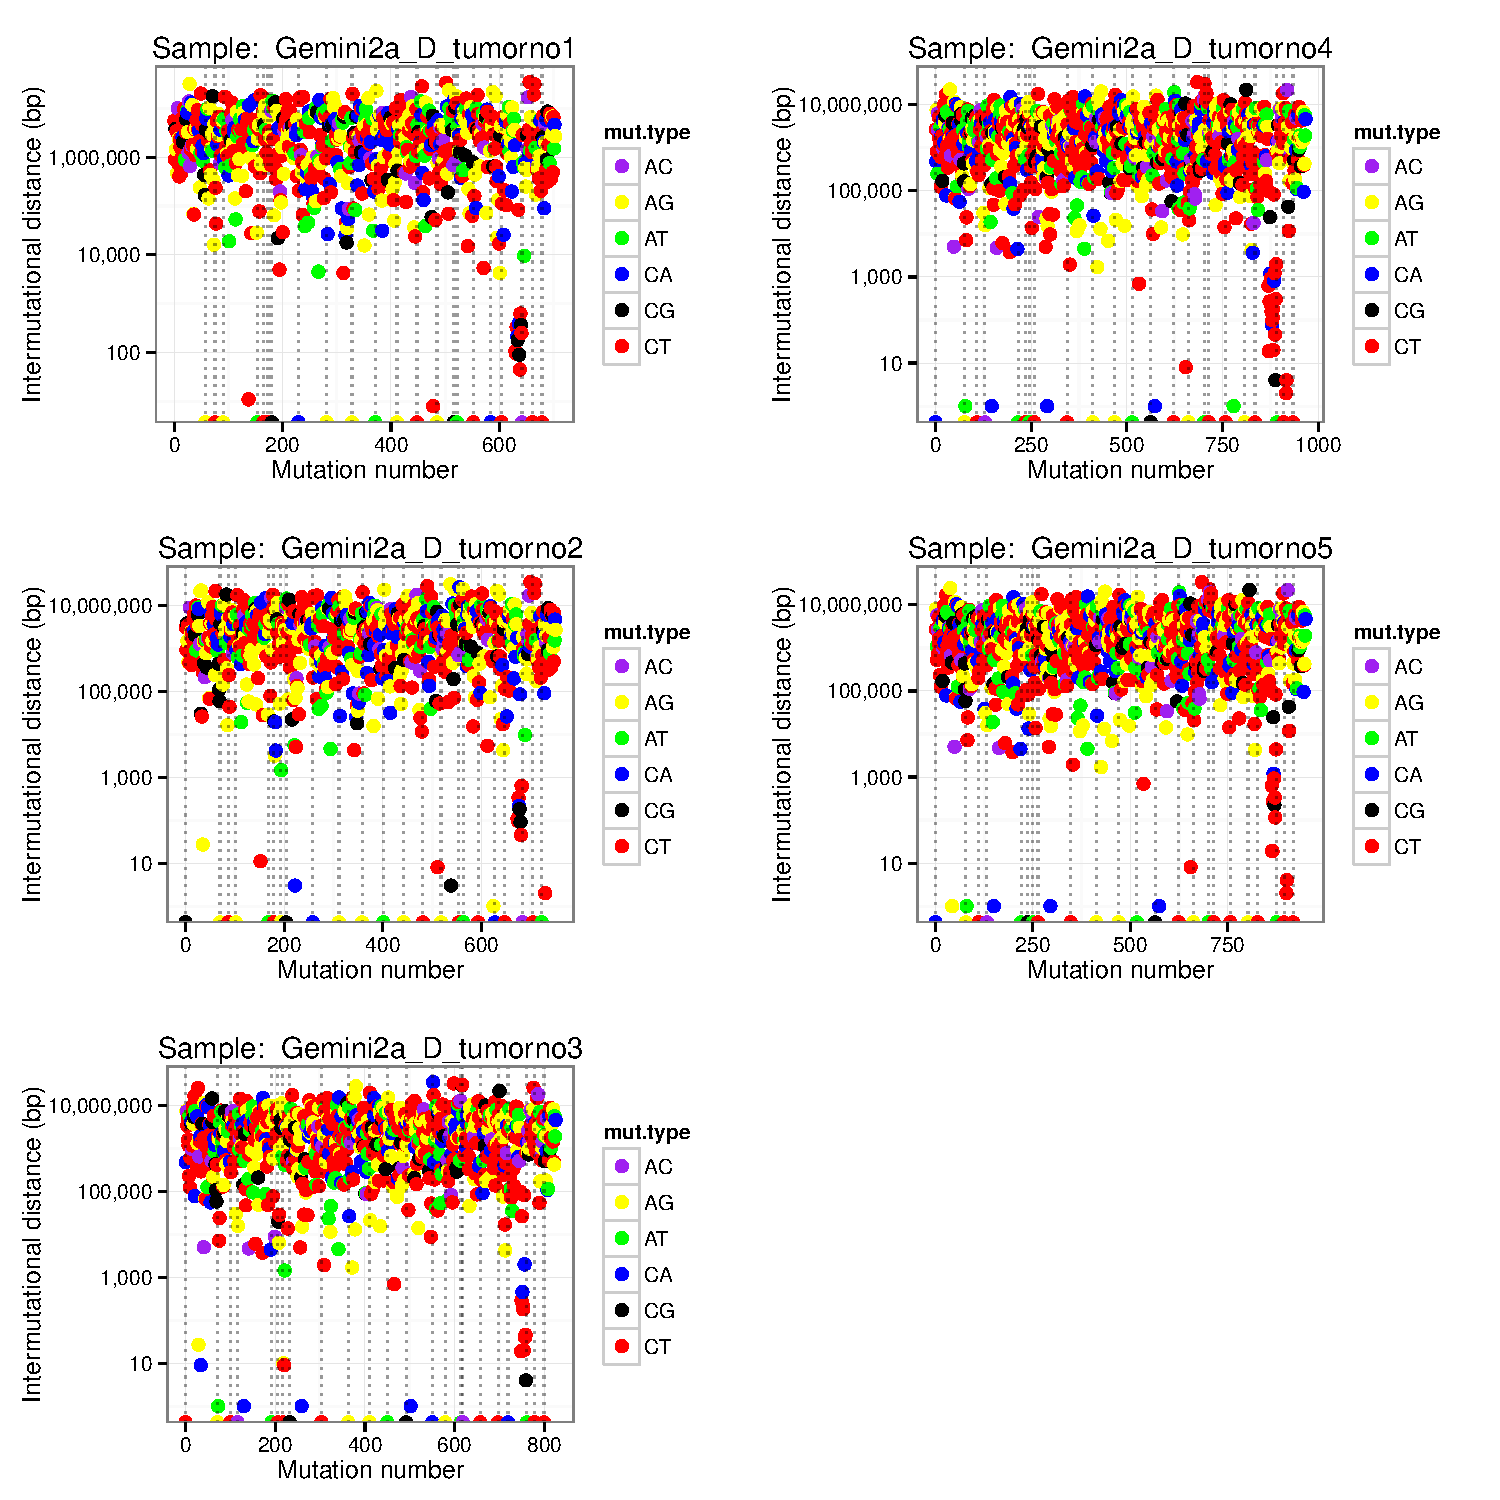
\includegraphics{CLLpilot_rainfallplots_pub-002}
\\
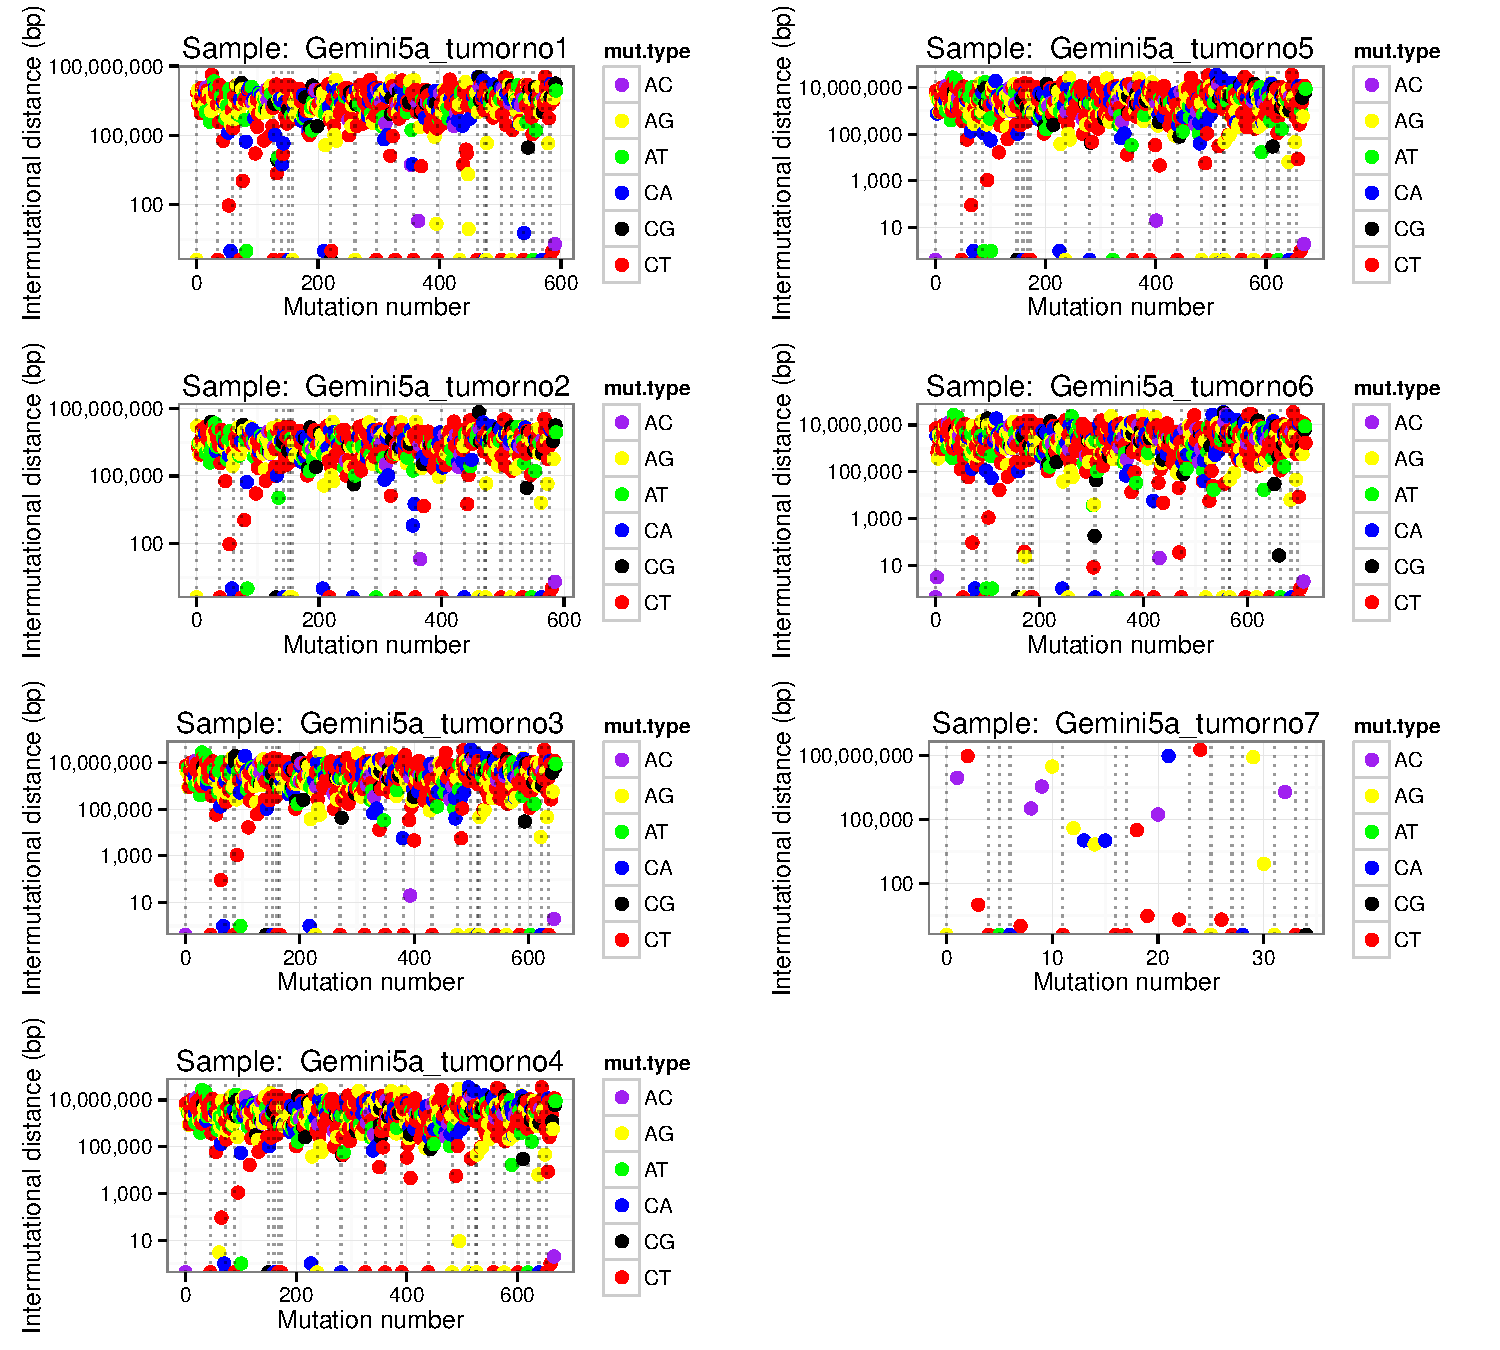
\includegraphics{CLLpilot_rainfallplots_pub-003}
\\
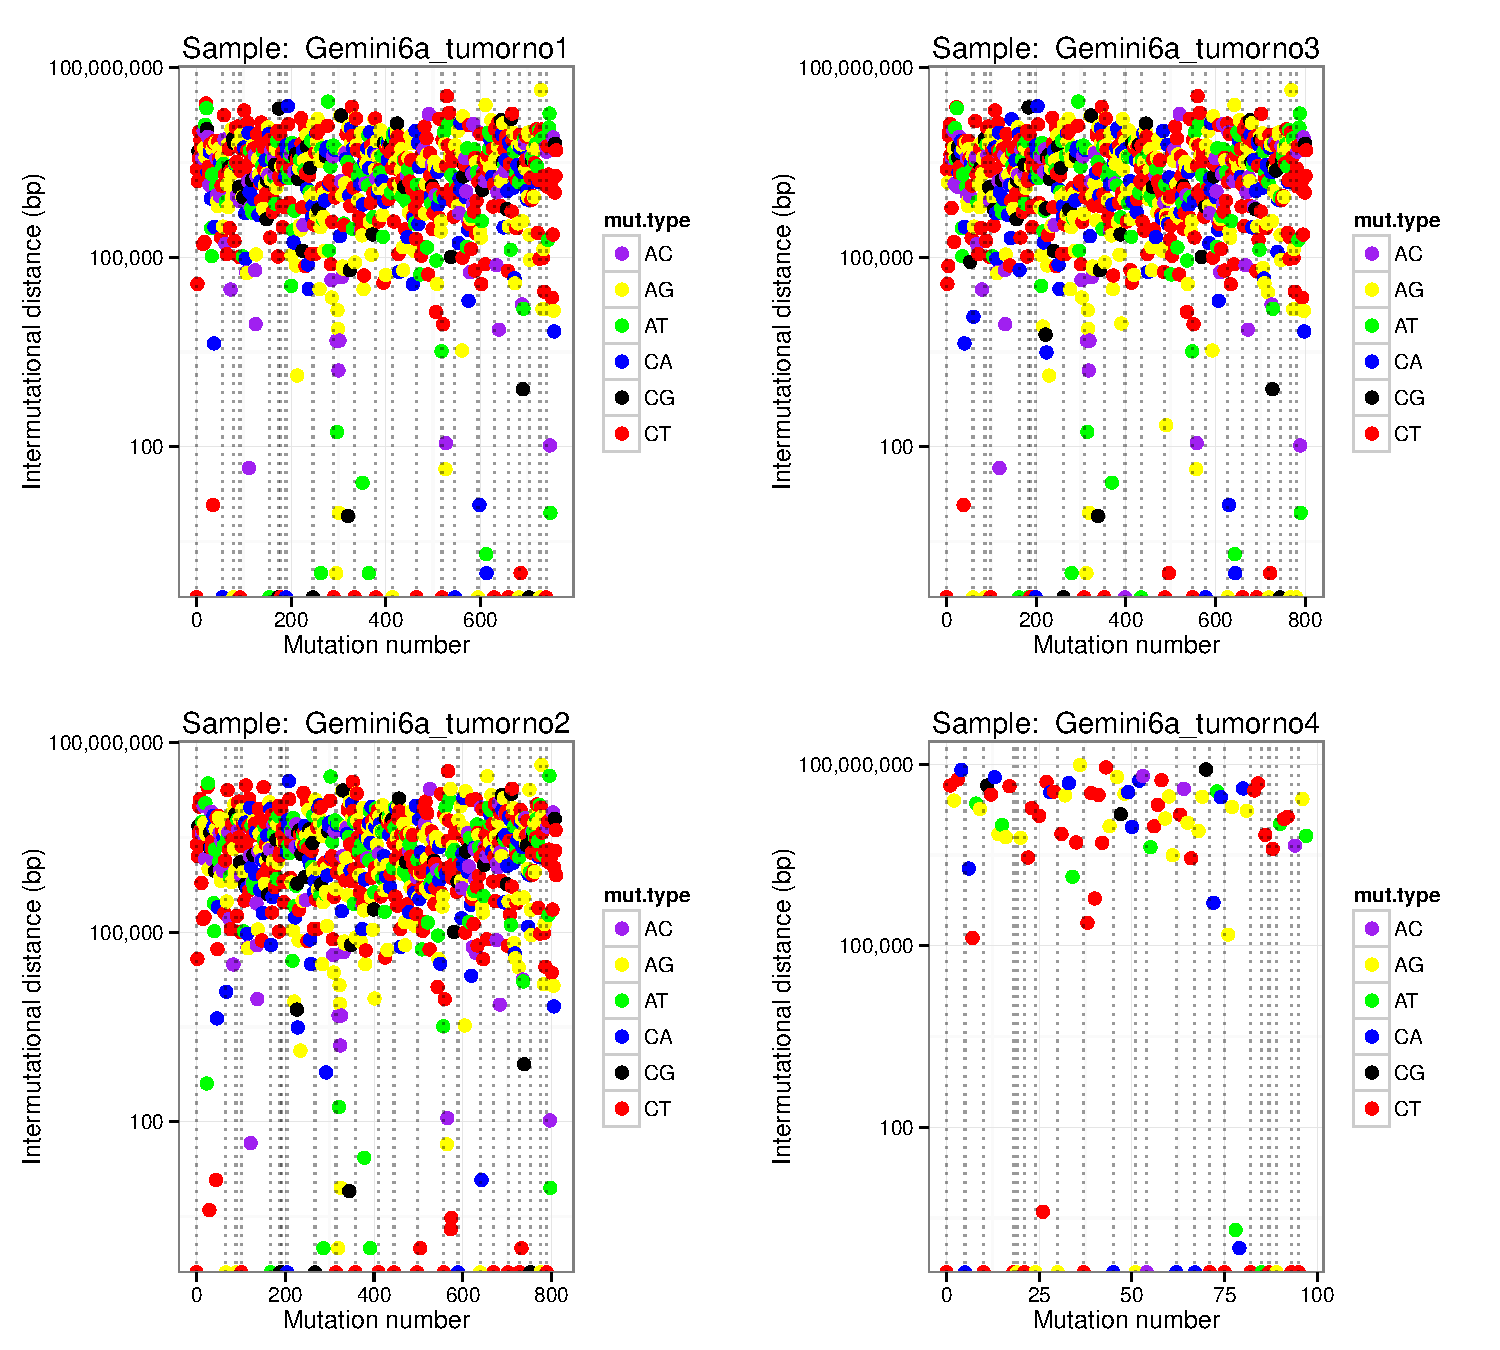
\includegraphics{CLLpilot_rainfallplots_pub-004}
\\
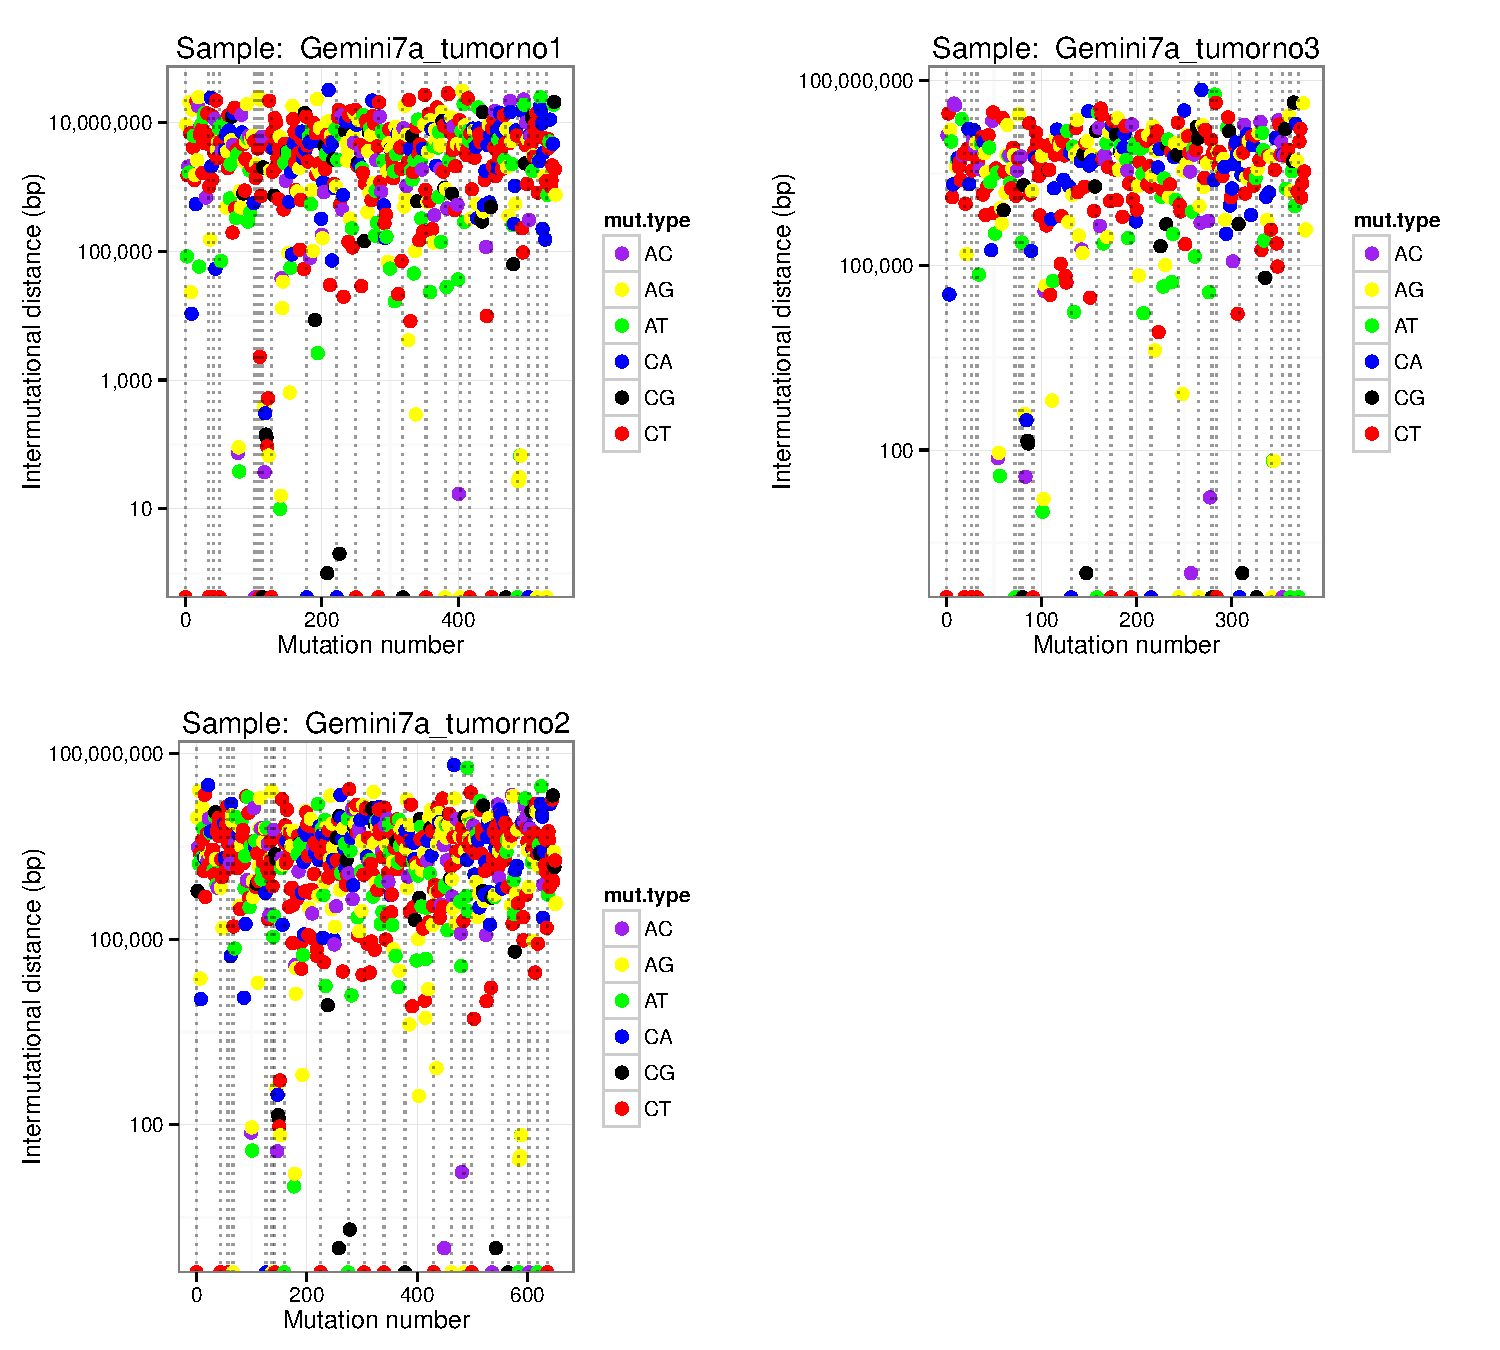
\includegraphics{CLLpilot_rainfallplots_pub-005}
\\
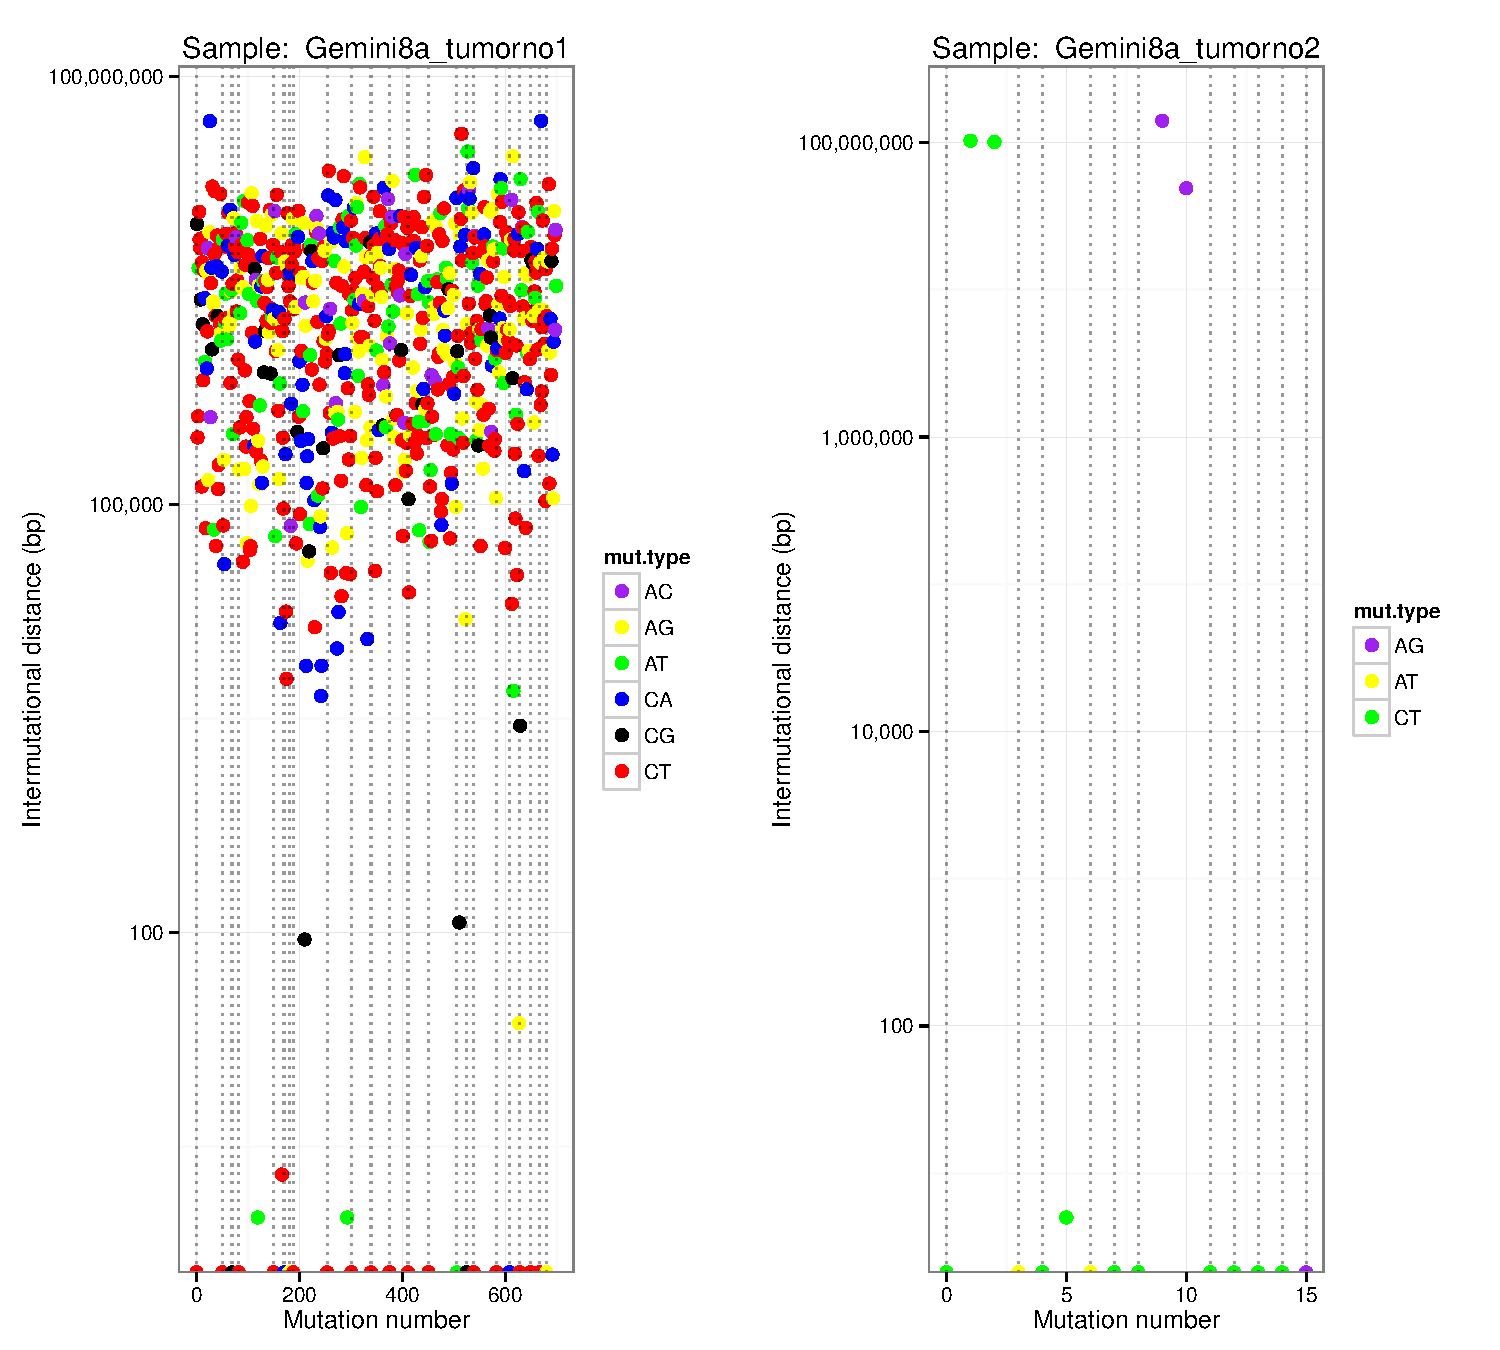
\includegraphics{CLLpilot_rainfallplots_pub-006}
\\
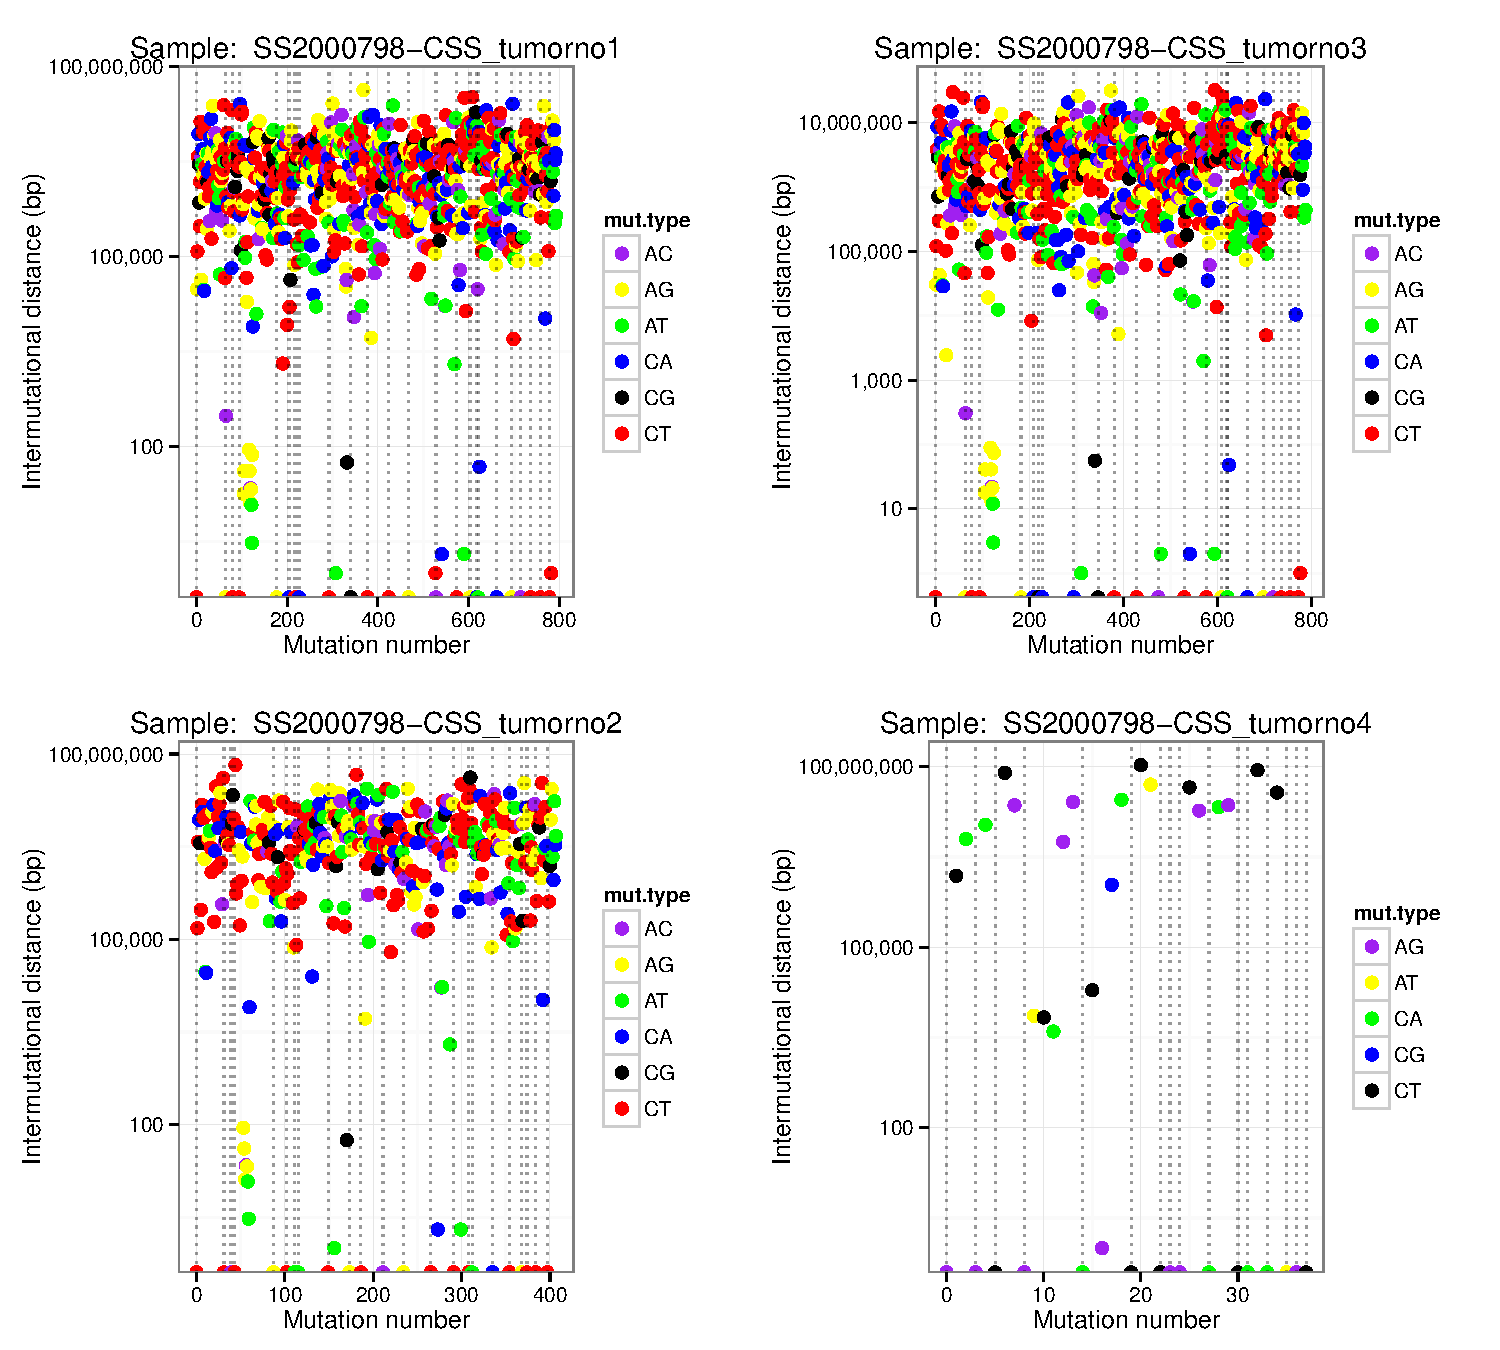
\includegraphics{CLLpilot_rainfallplots_pub-007}
\\
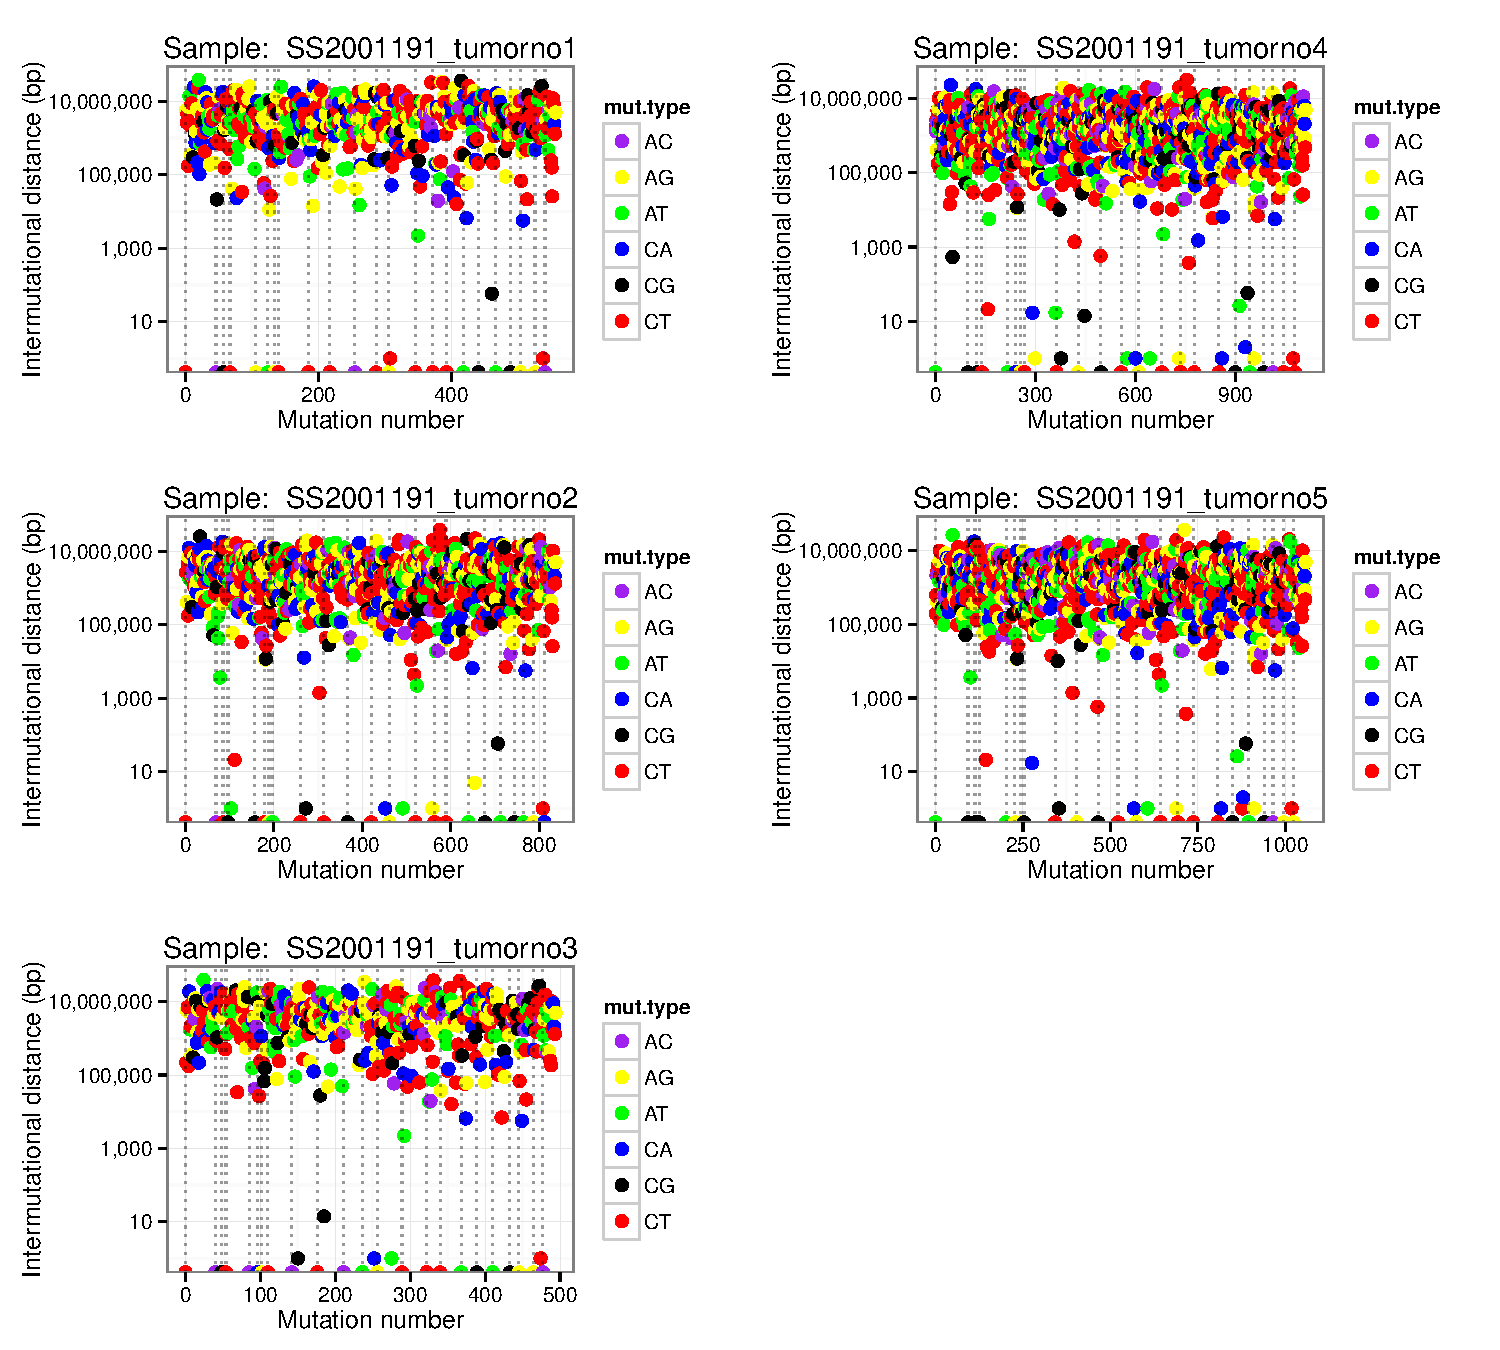
\includegraphics{CLLpilot_rainfallplots_pub-008}
\\
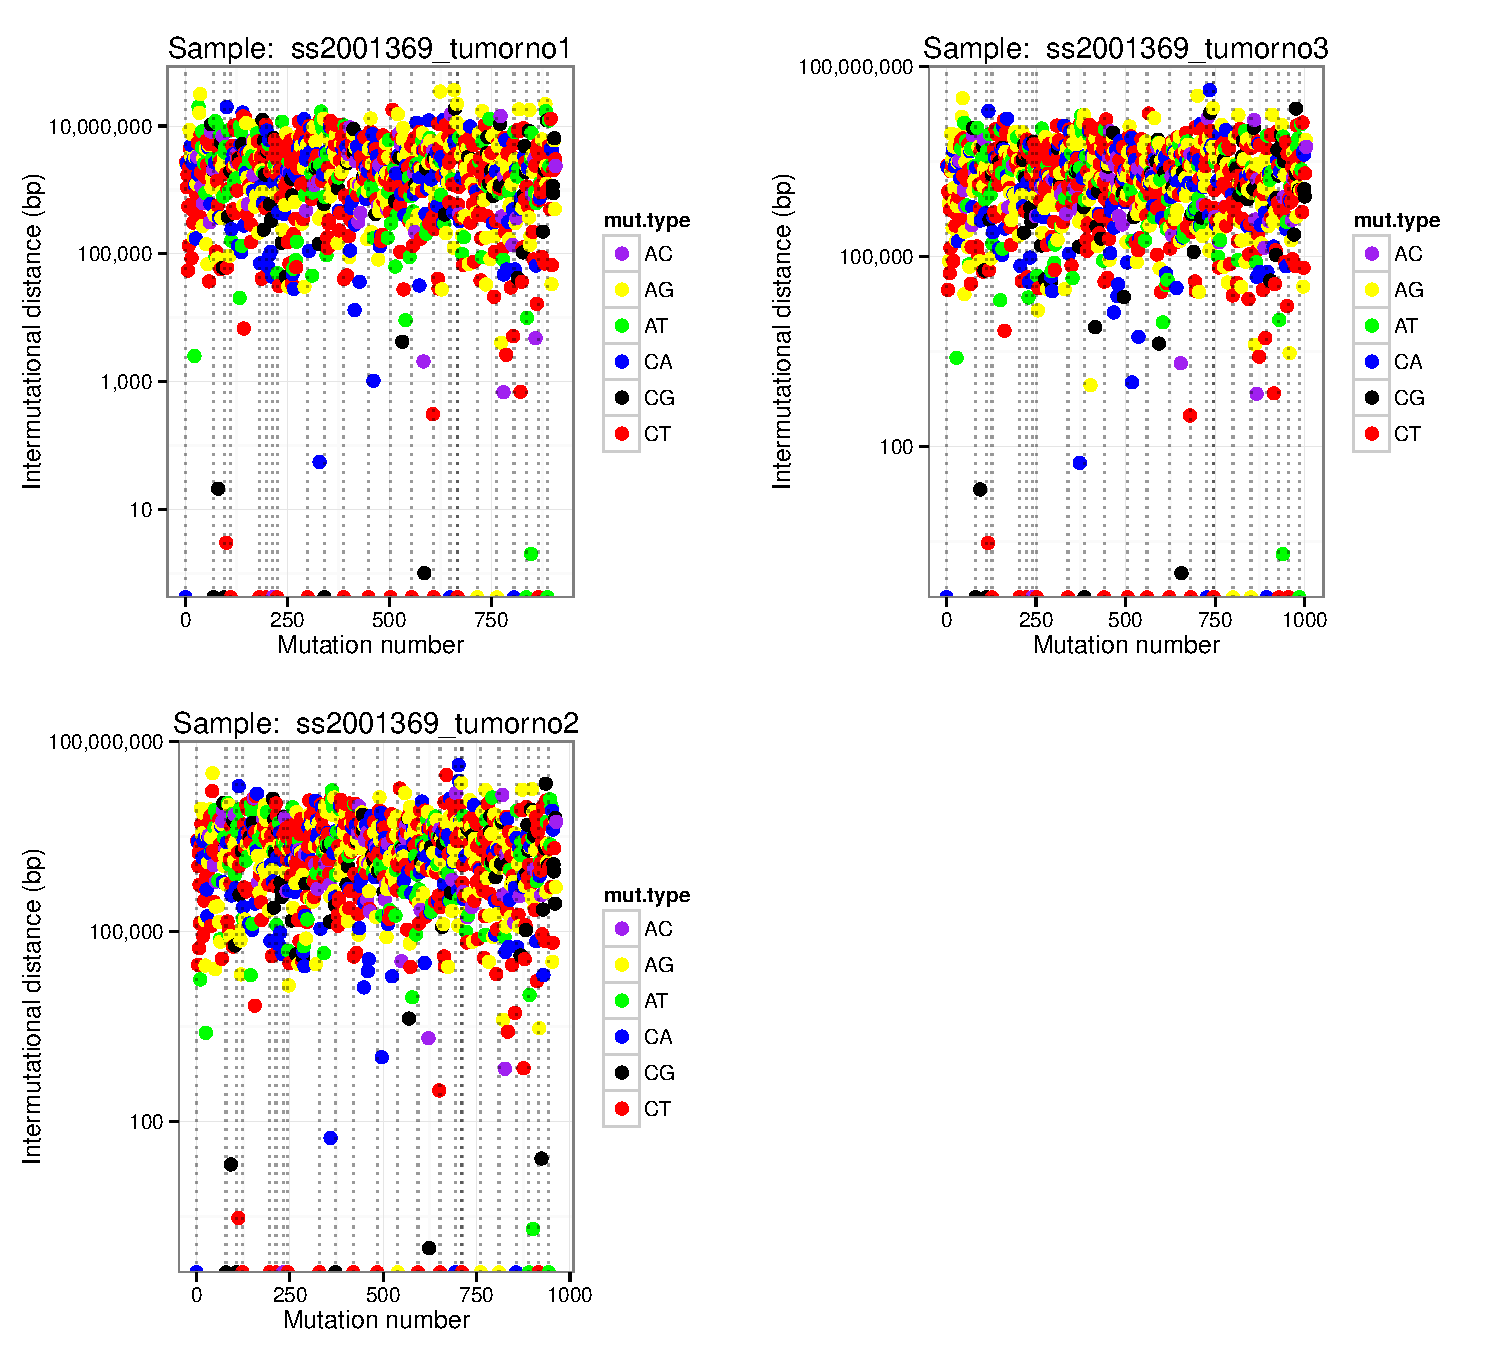
\includegraphics{CLLpilot_rainfallplots_pub-009}
\\
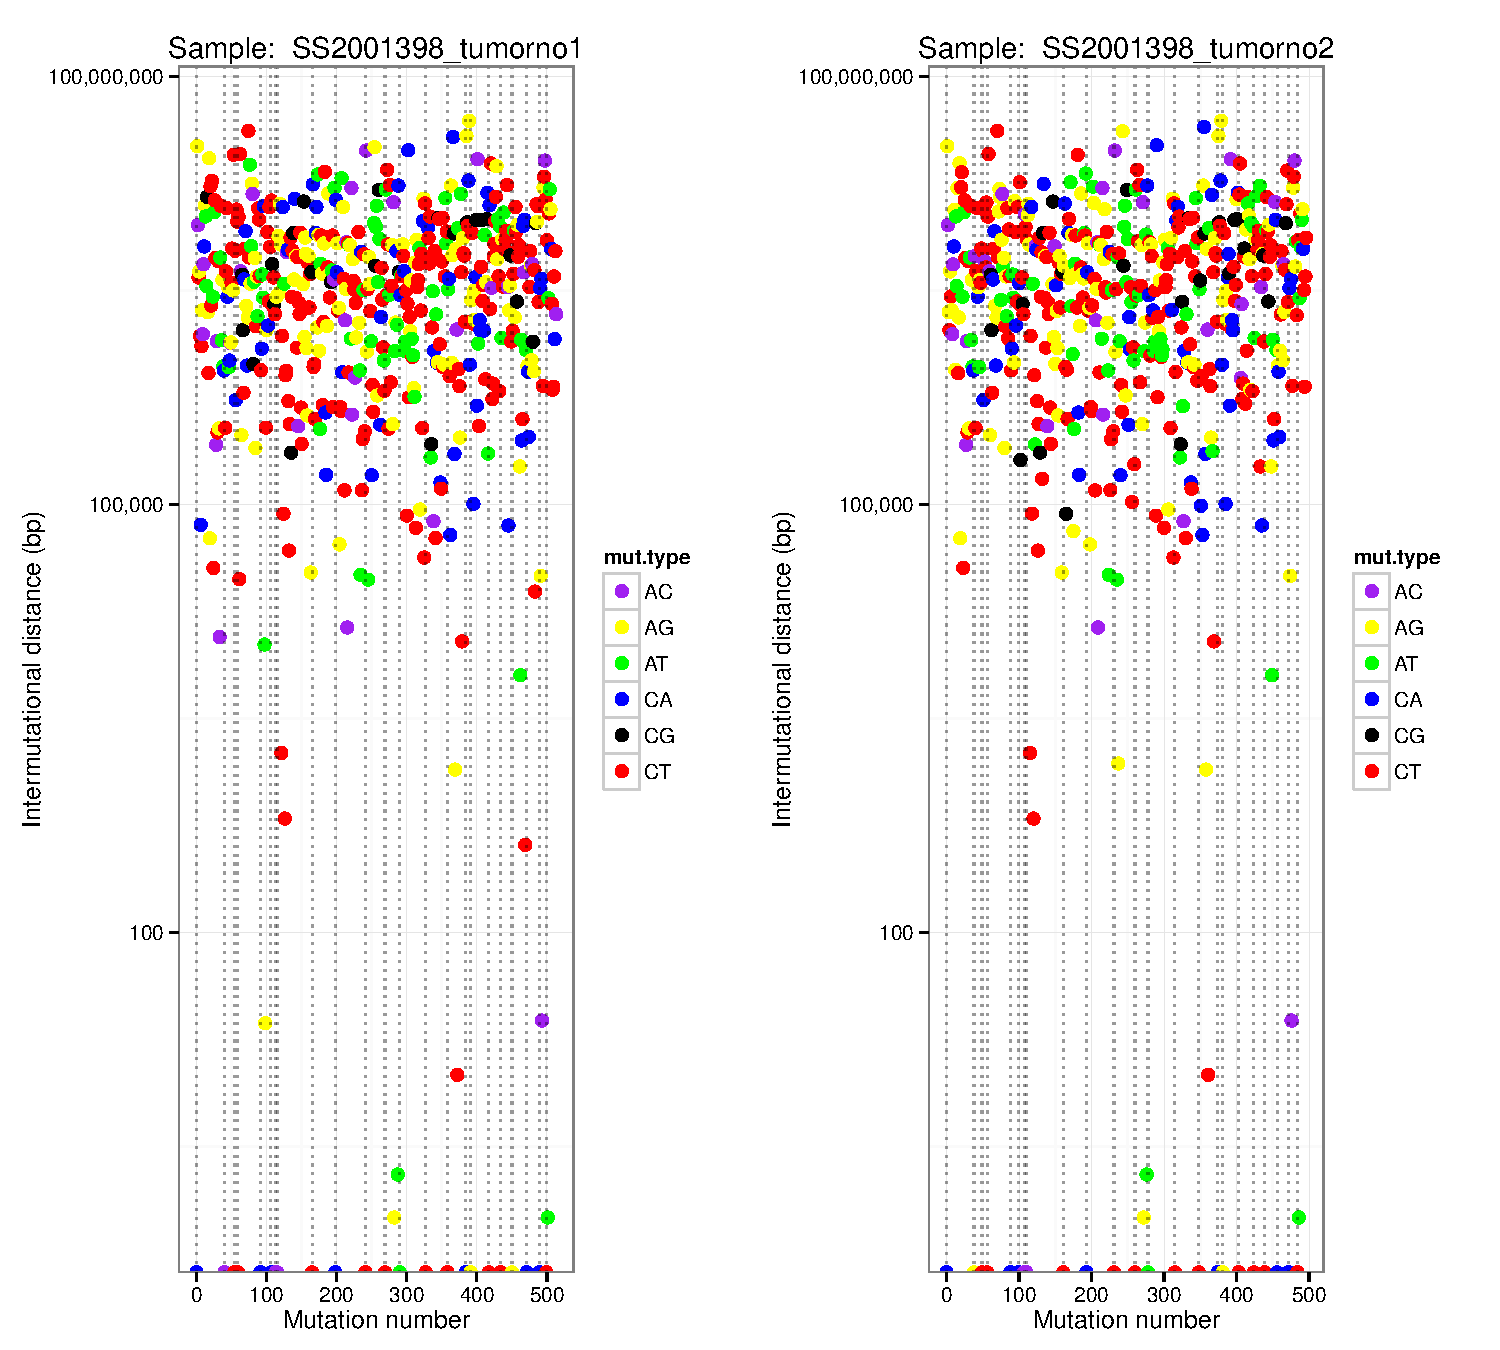
\includegraphics{CLLpilot_rainfallplots_pub-010}
\\
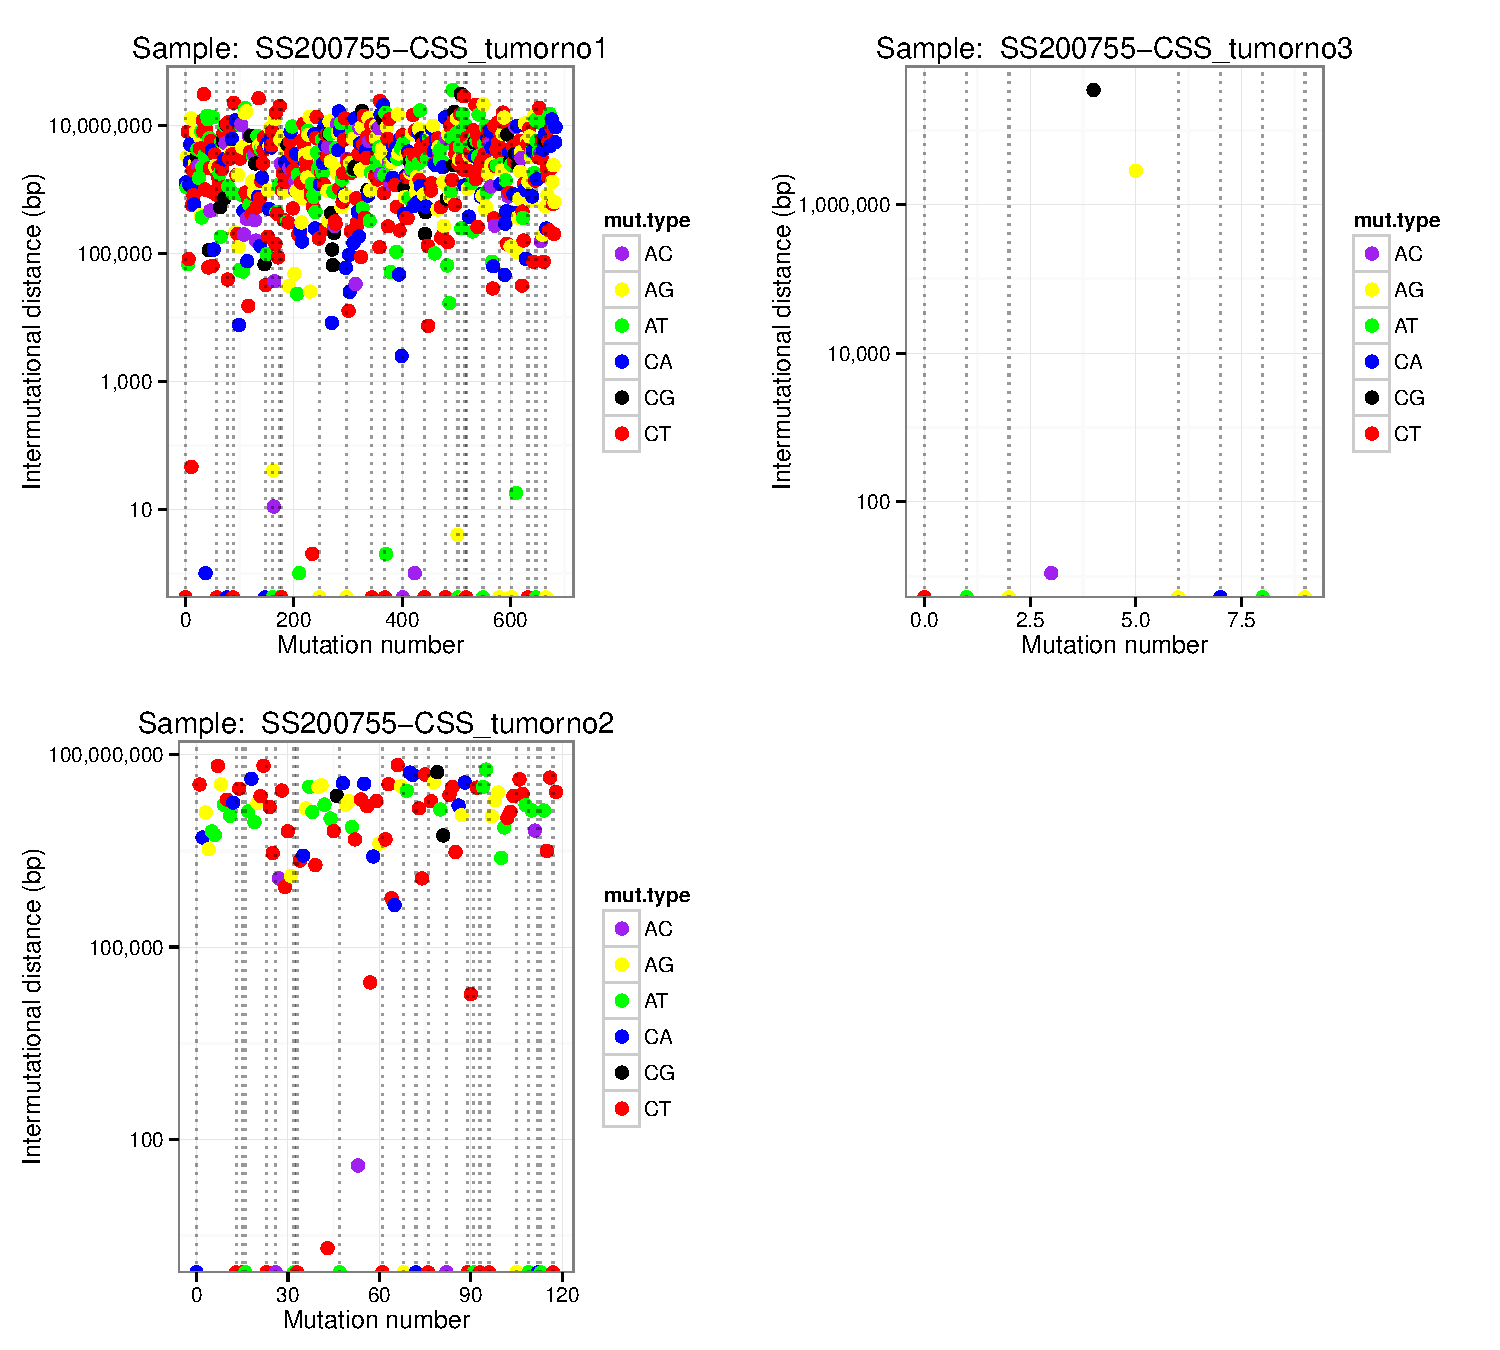
\includegraphics{CLLpilot_rainfallplots_pub-011}
\section{Number of Kataegis events}
From Lawrence 2013, nature:\\
"Kataegis events, detected by identifying stretches of at least six mutations having inter-mutation distances at least two standard deviations smaller than the sample median, are indicated with blue boxes at the bottom of the plots. In some cases it can be observed that the individual mutations of a kataegis event are all of the same category."\\
Because we have a very low number of kataegis events anyway, I counted each event separately, using the 10\% quantile as a cutoff. Note that the low number of kataegis events in some of the final samples might come from germ line contaminations.


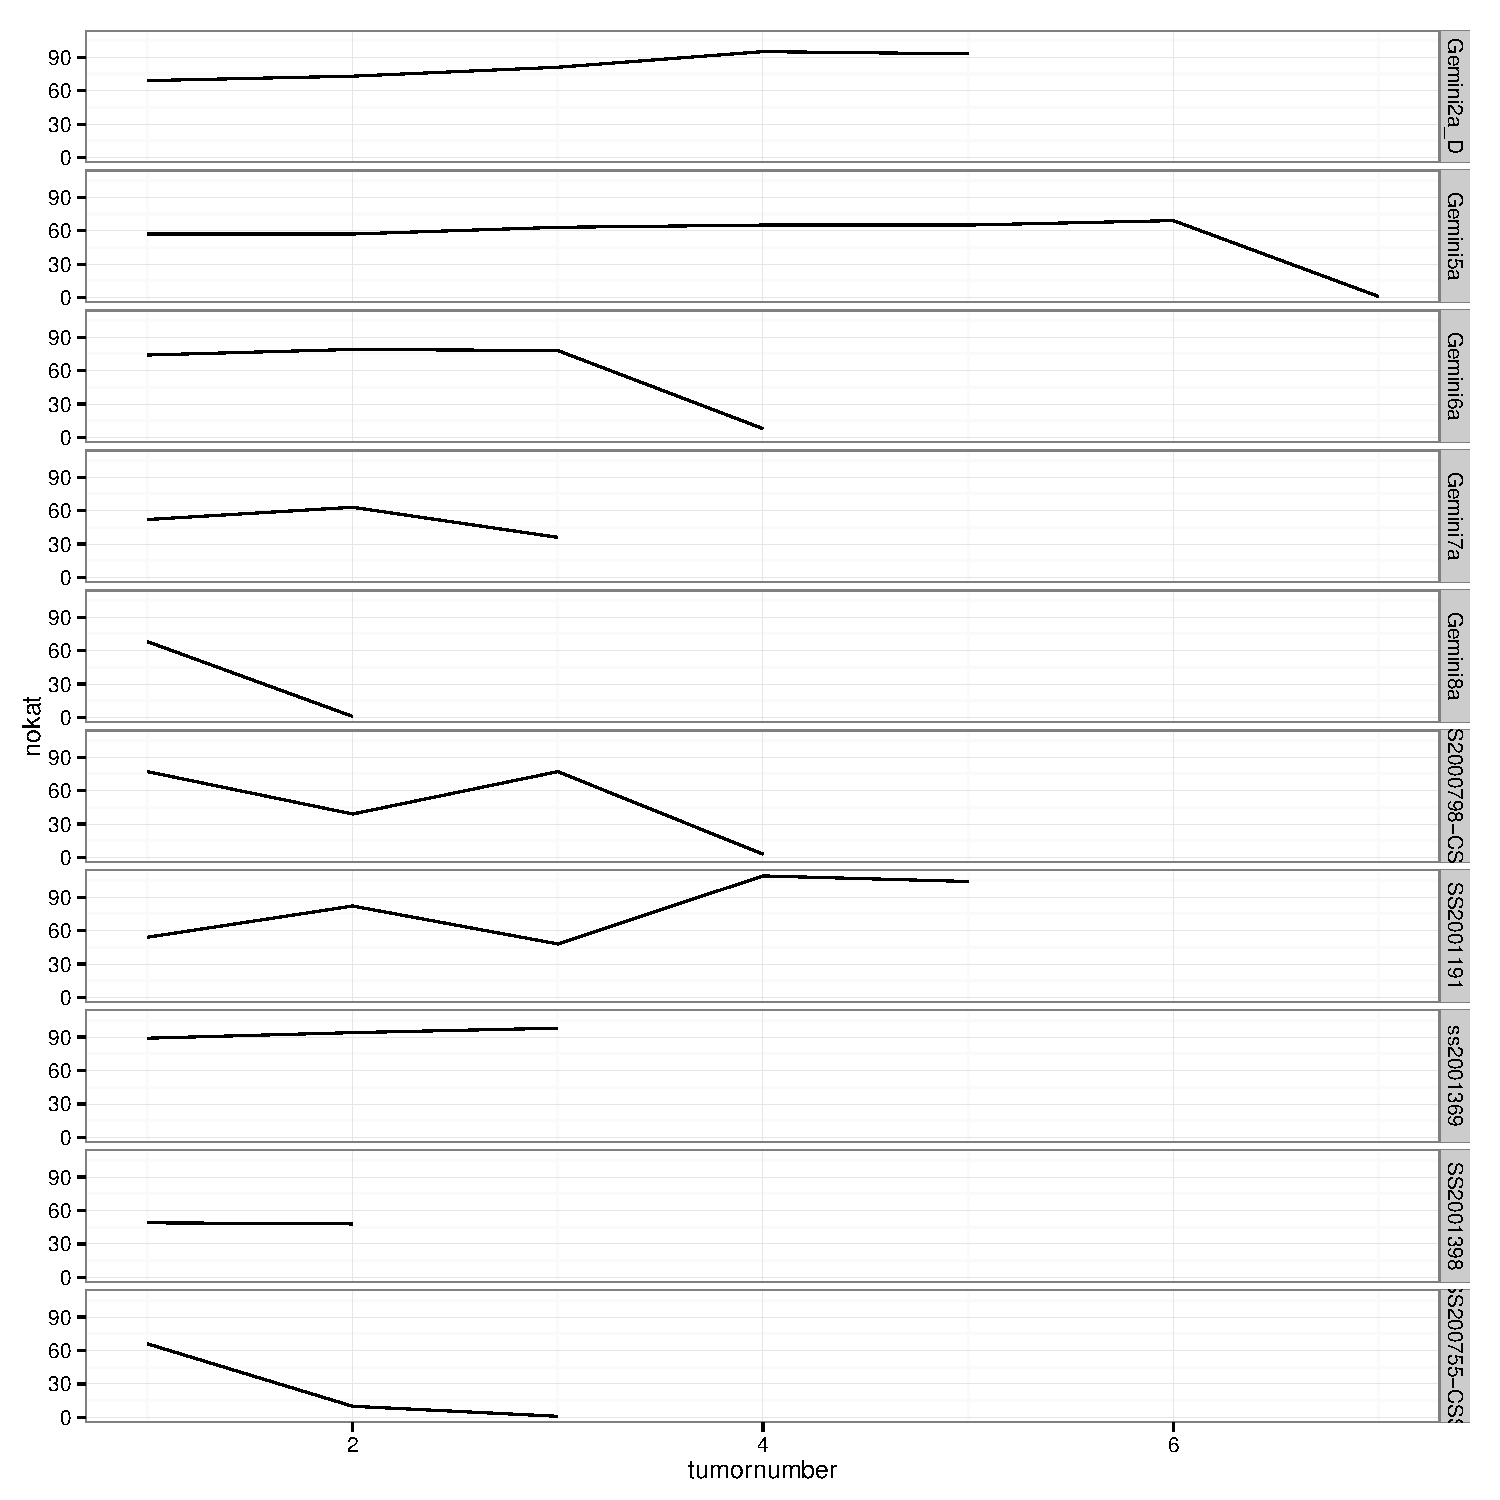
\includegraphics{CLLpilot_rainfallplots_pub-013}

\end{document}
